\documentclass[11pt]{article}
%Gummi|063|=)
\title{\textbf{The fabrik of knowledge}}
\usepackage{graphicx}
\usepackage{amsmath}
\begin{document}
\maketitle


\section{smallest part of what we call knowledge}
The picture shows an assemblage of concepts as they look when plotted with GraphViz.
Its a bit like snow as every concept has a different structure,
some simple ones some complex generally a concept can have one ore more 
exits which lead into one or more related concepts like\\
( I'm going = to the shop // crazy )

using graph wizard for sampling concepts one level only!!!


\begin{figure}[htp]
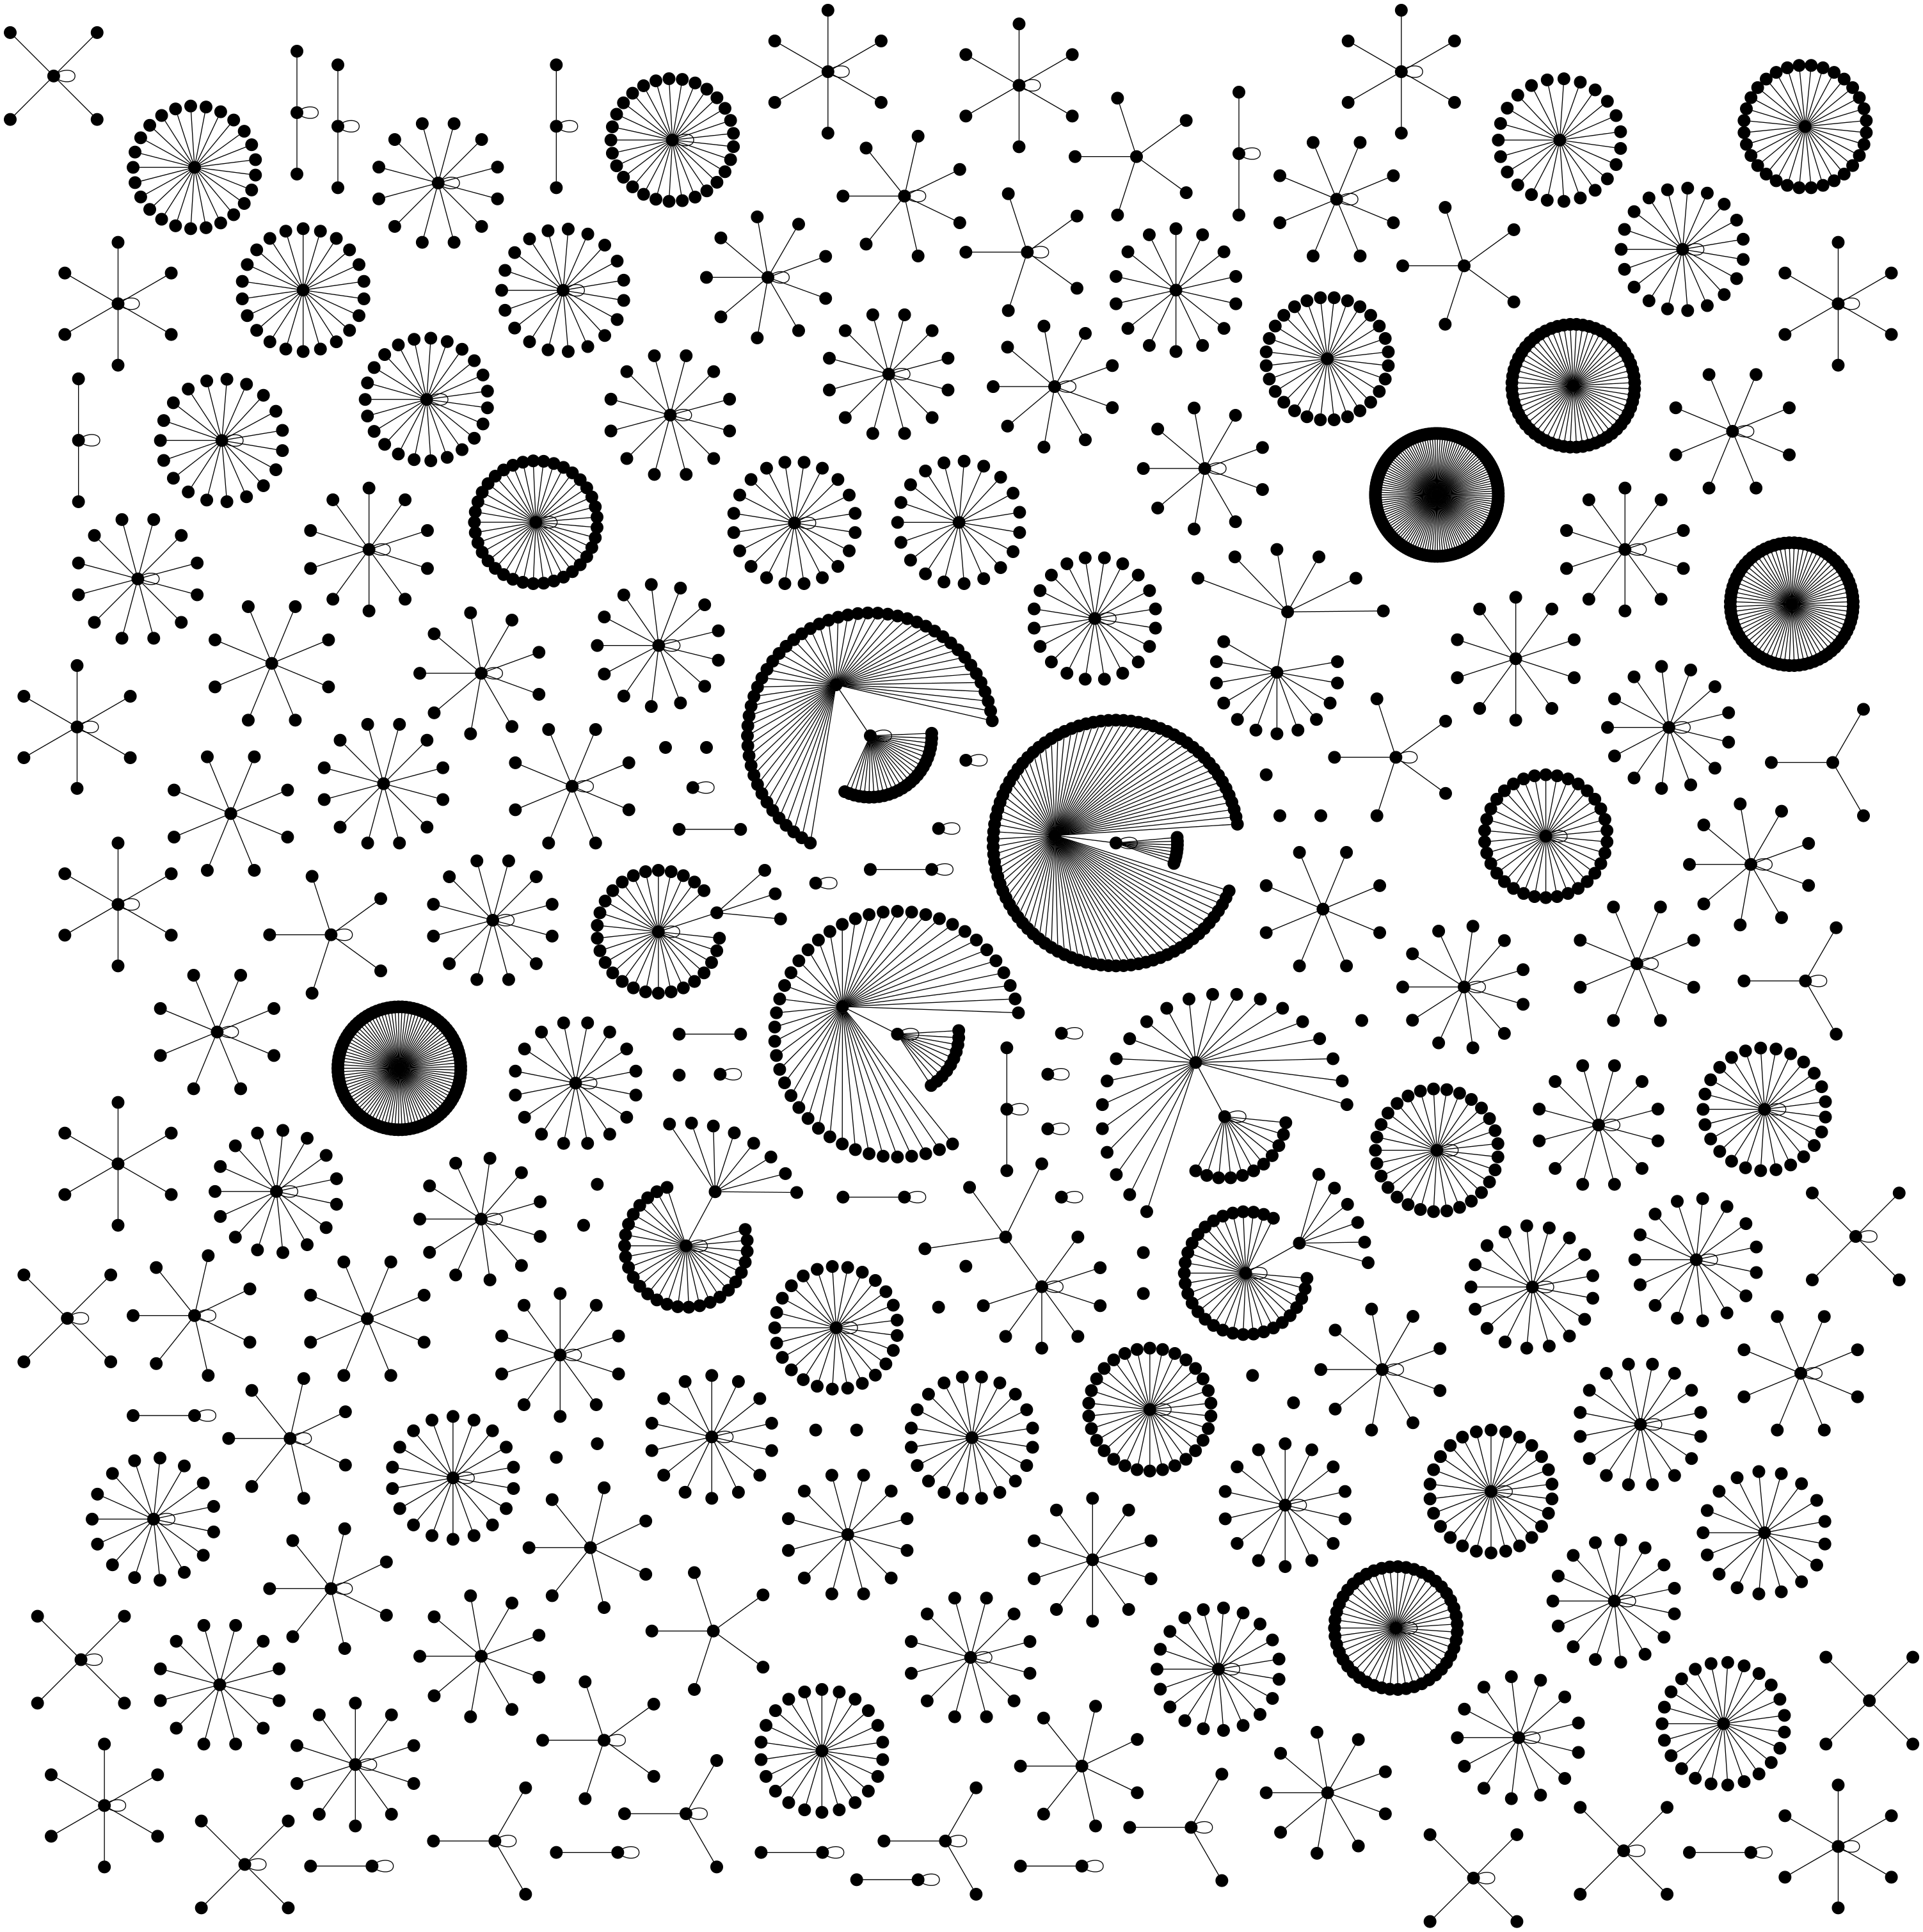
\includegraphics[scale=0.08]{img/a_directories.png}
\caption{generating fairly random concepts with common letter [a] }
\label{}
\end{figure}



\section{A knowledge system }

A large number of concepts even if assembled randomly 
will form a system where the relations will form connections 
which would make it possible to move from one concept to any other within 
the system.


\begin{figure}[htp]
\centering
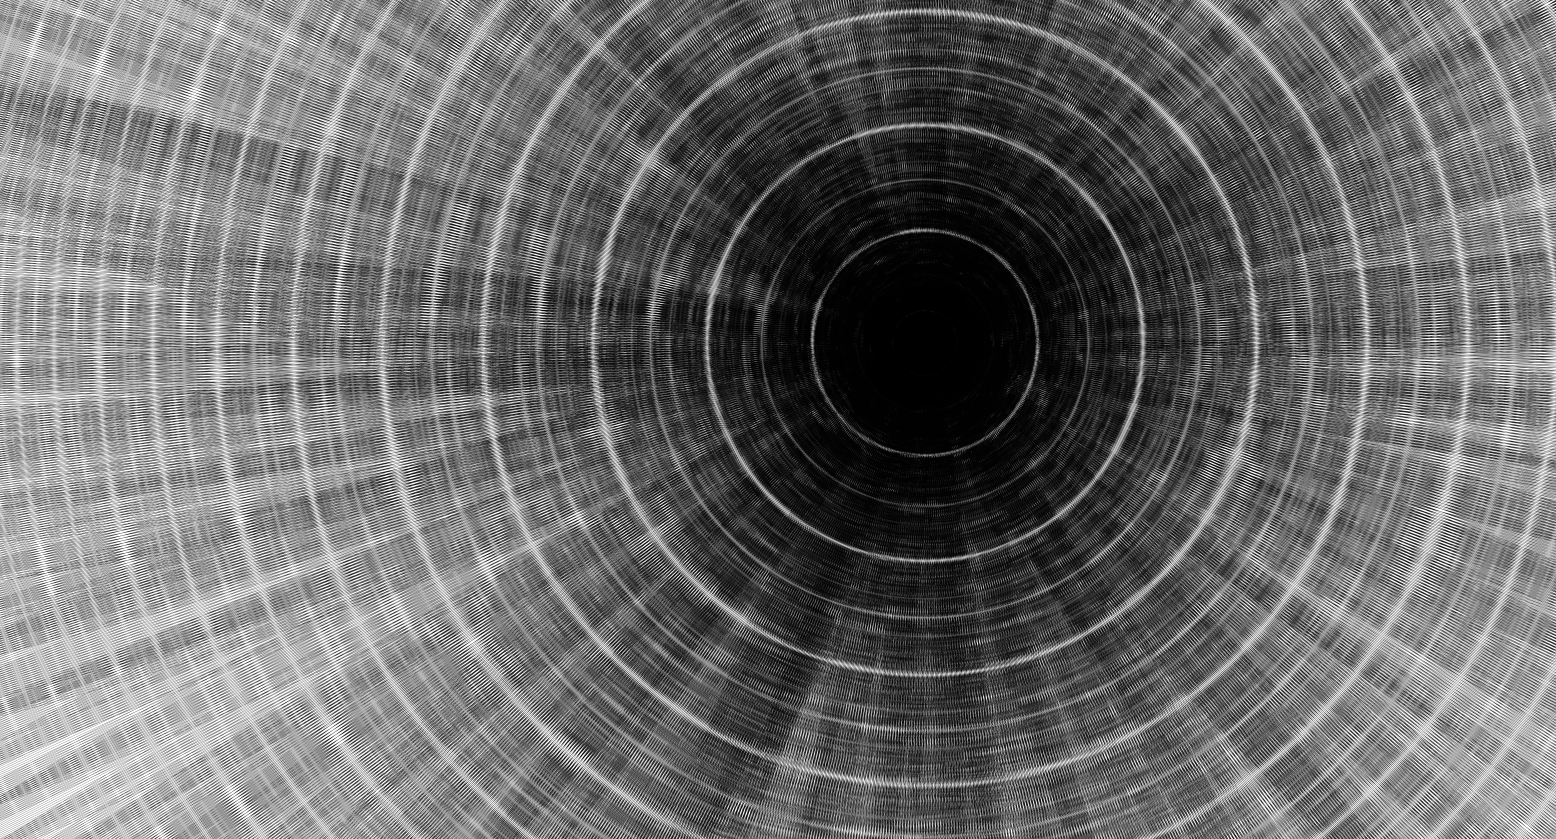
\includegraphics[scale=0.25]{img/1362924302_directories.png}
\caption{knowledge system with round about 1k concepts}
\label{every thought is interlocked somewhere at some point}
\end{figure}





\section{Making knowledge}
Lets start to render something simple like 
fiction


          \begin{verbatim}
AI::MicroStructure::ObjectSet  {
    public methods (11) : check, decruft, domain, final, includes, includes_name, insert, members, new, retrieve, size
    private methods (0)
    internals: {
        fiction               AI::MicroStructure::Object,
        fictional             AI::MicroStructure::Object,
        fictional_animal      AI::MicroStructure::Object,
        fictional_character   AI::MicroStructure::Object,
        fictionalisation      AI::MicroStructure::Object,
        fictionalise          AI::MicroStructure::Object,
        fictionalization      AI::MicroStructure::Object,
        fictionalize          AI::MicroStructure::Object,
        micro                 [],
        obj                   {
            center   {
                fiction                        1,
                fictional                      2,
                fictional_animal               3,
                fictional_character            3,
                fictional_(vs._nonfictional)   2,
                fictionalisation               3,
                fictionalise                   3,
                fictionalization               3,
                fictionalize                   3,
                science_fiction                2
            },
            dense    {
                fictional_animal      3,
                fictional_character   3,
                fictionalisation      3,
                fictionalise          3,
                fictionalization      3,
                fictionalize          3
            },
            domain   "fiction_5641b1121c44f4929fde6b274d164e60",
            IN       [],
            max      3,
            mean     2.3,
            menu     {
                fictional_animal      3,
                fictional_character   3,
                fictionalisation      3,
                fictionalise          3,
                fictionalization      3,
                fictionalize          3
            },
            min      3
        },
        science_fiction       AI::MicroStructure::Object
    }
}

real    0m0.163s
user    0m0.140s
sys     0m0.016s

So we would now have a seed knowledge system which we could expand from


          \end{verbatim}


\section{Pictures}




\begin{figure}[htp]
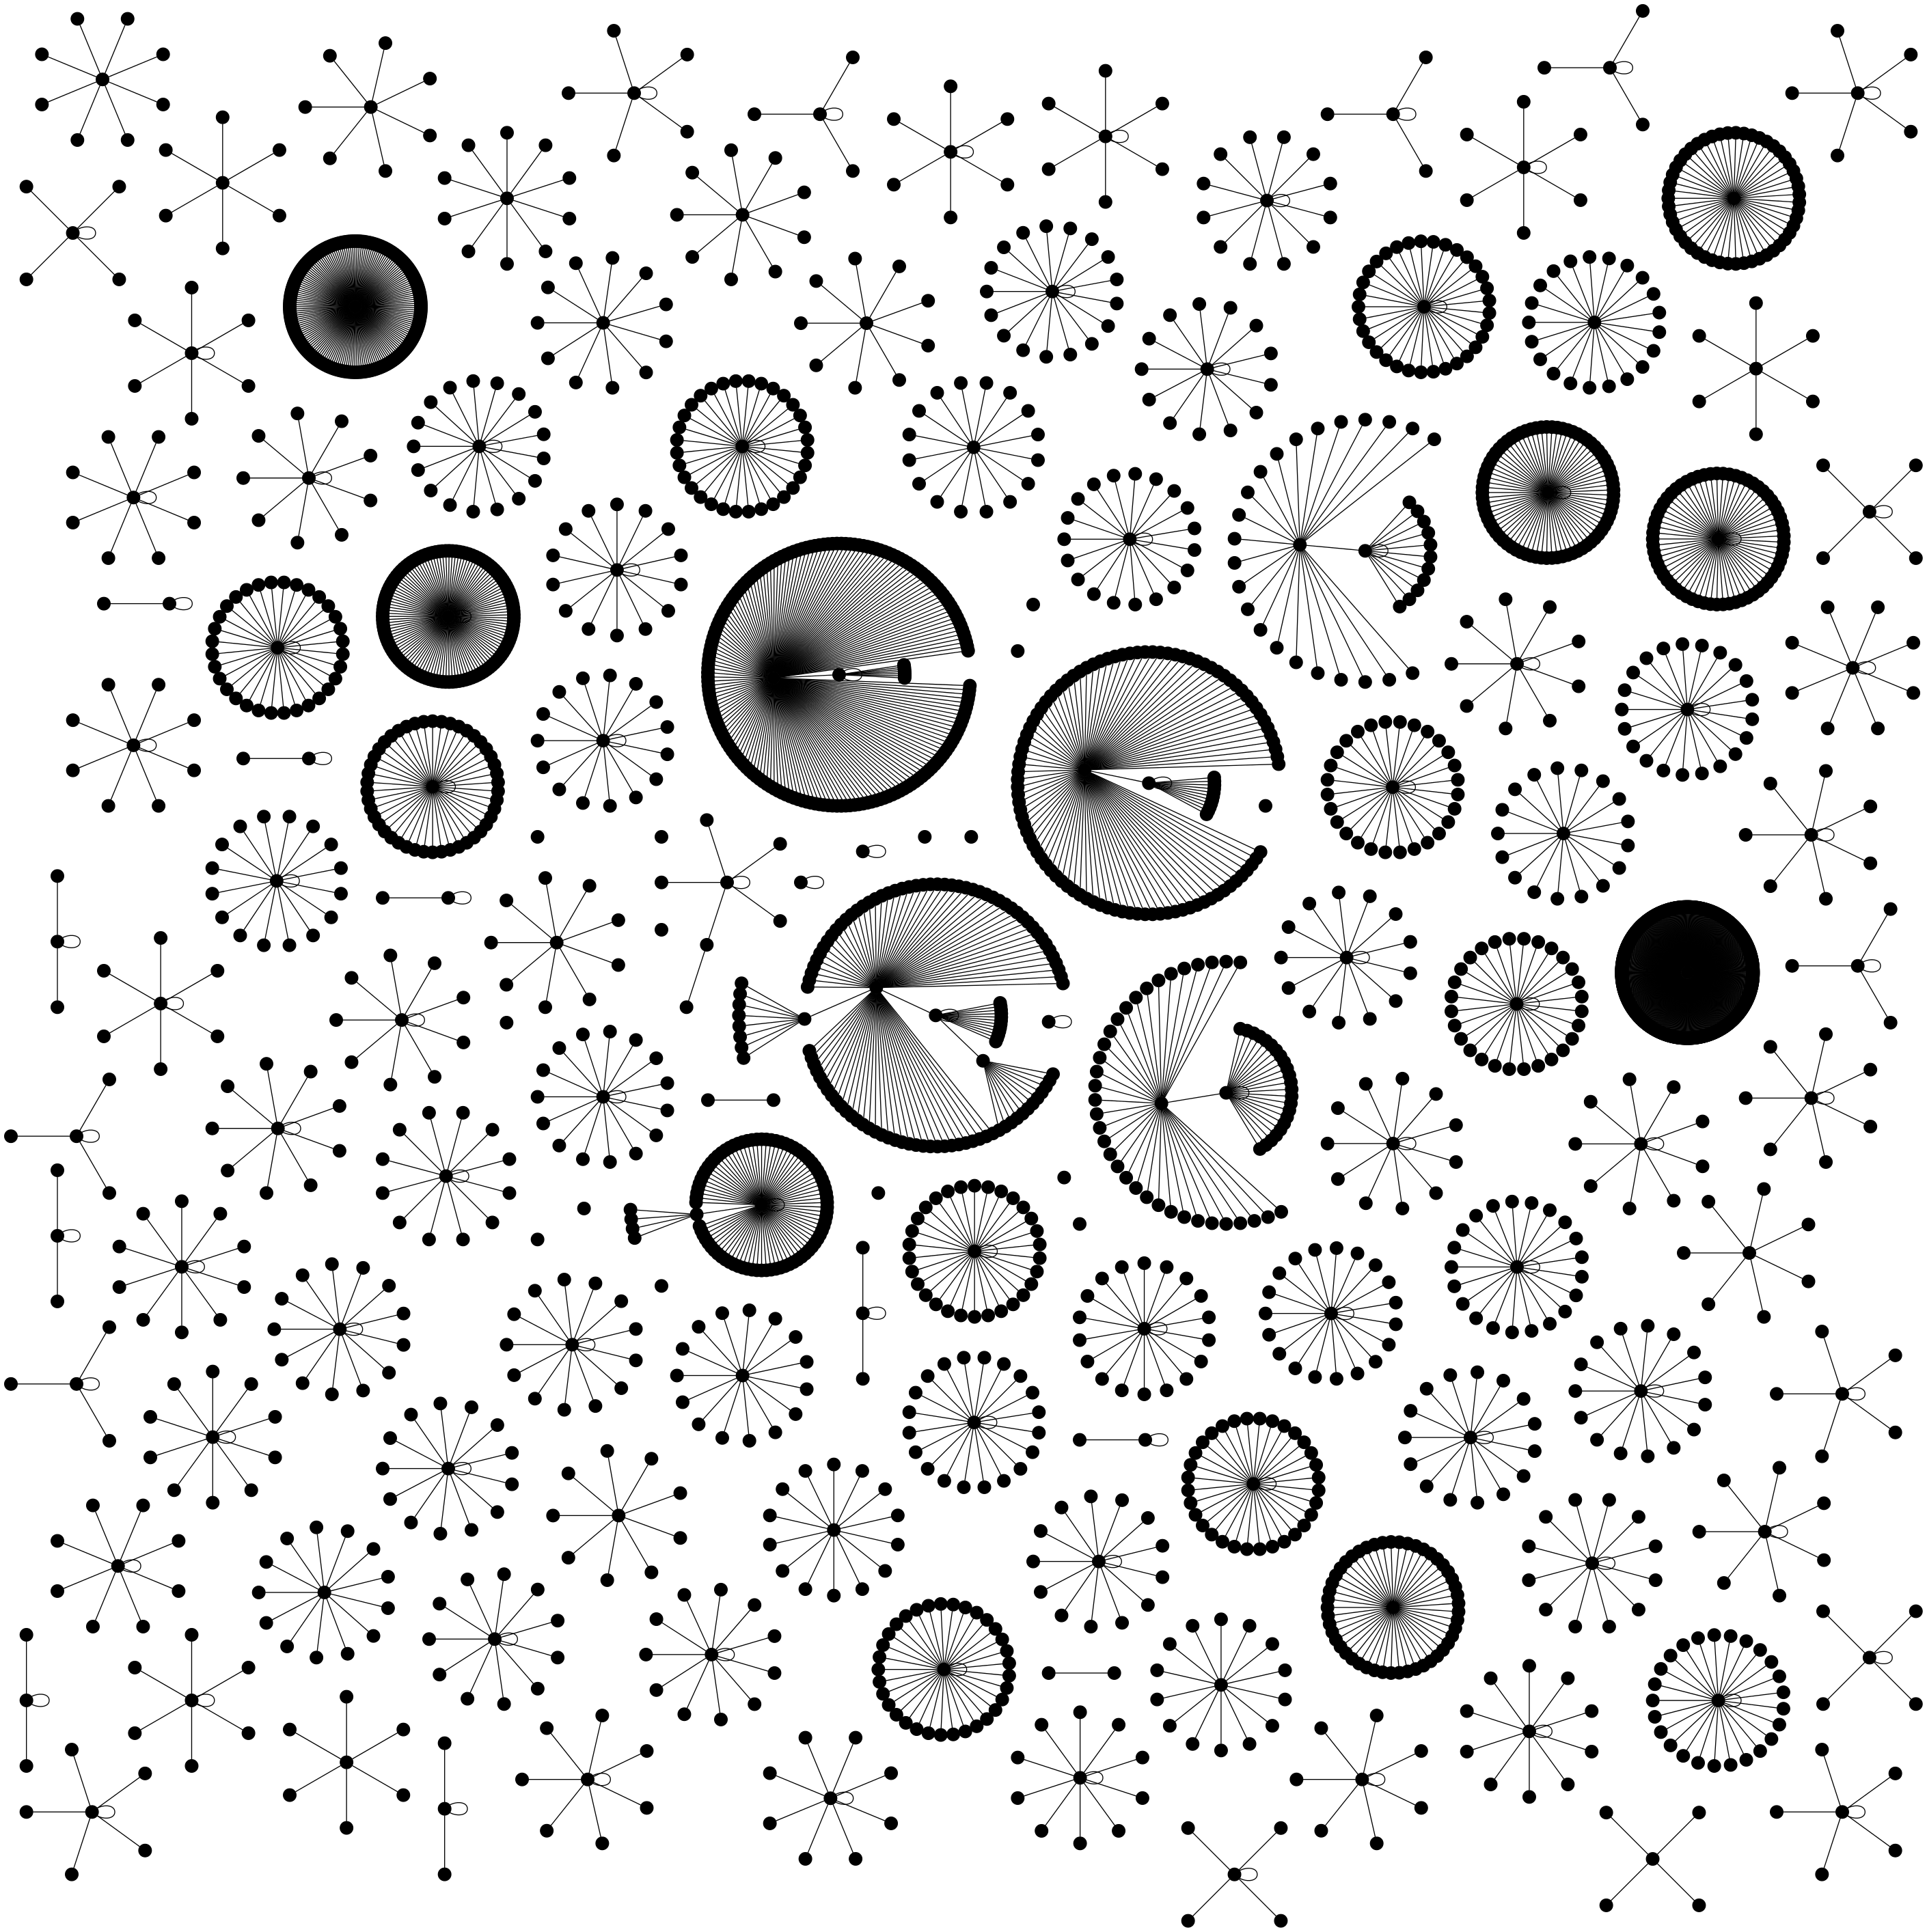
\includegraphics[scale=0.10]{img/m_directories.png}
\caption{a random generation of unrelated concepts}
\label{}
\end{figure}




common character [w]

\begin{figure}[htp]
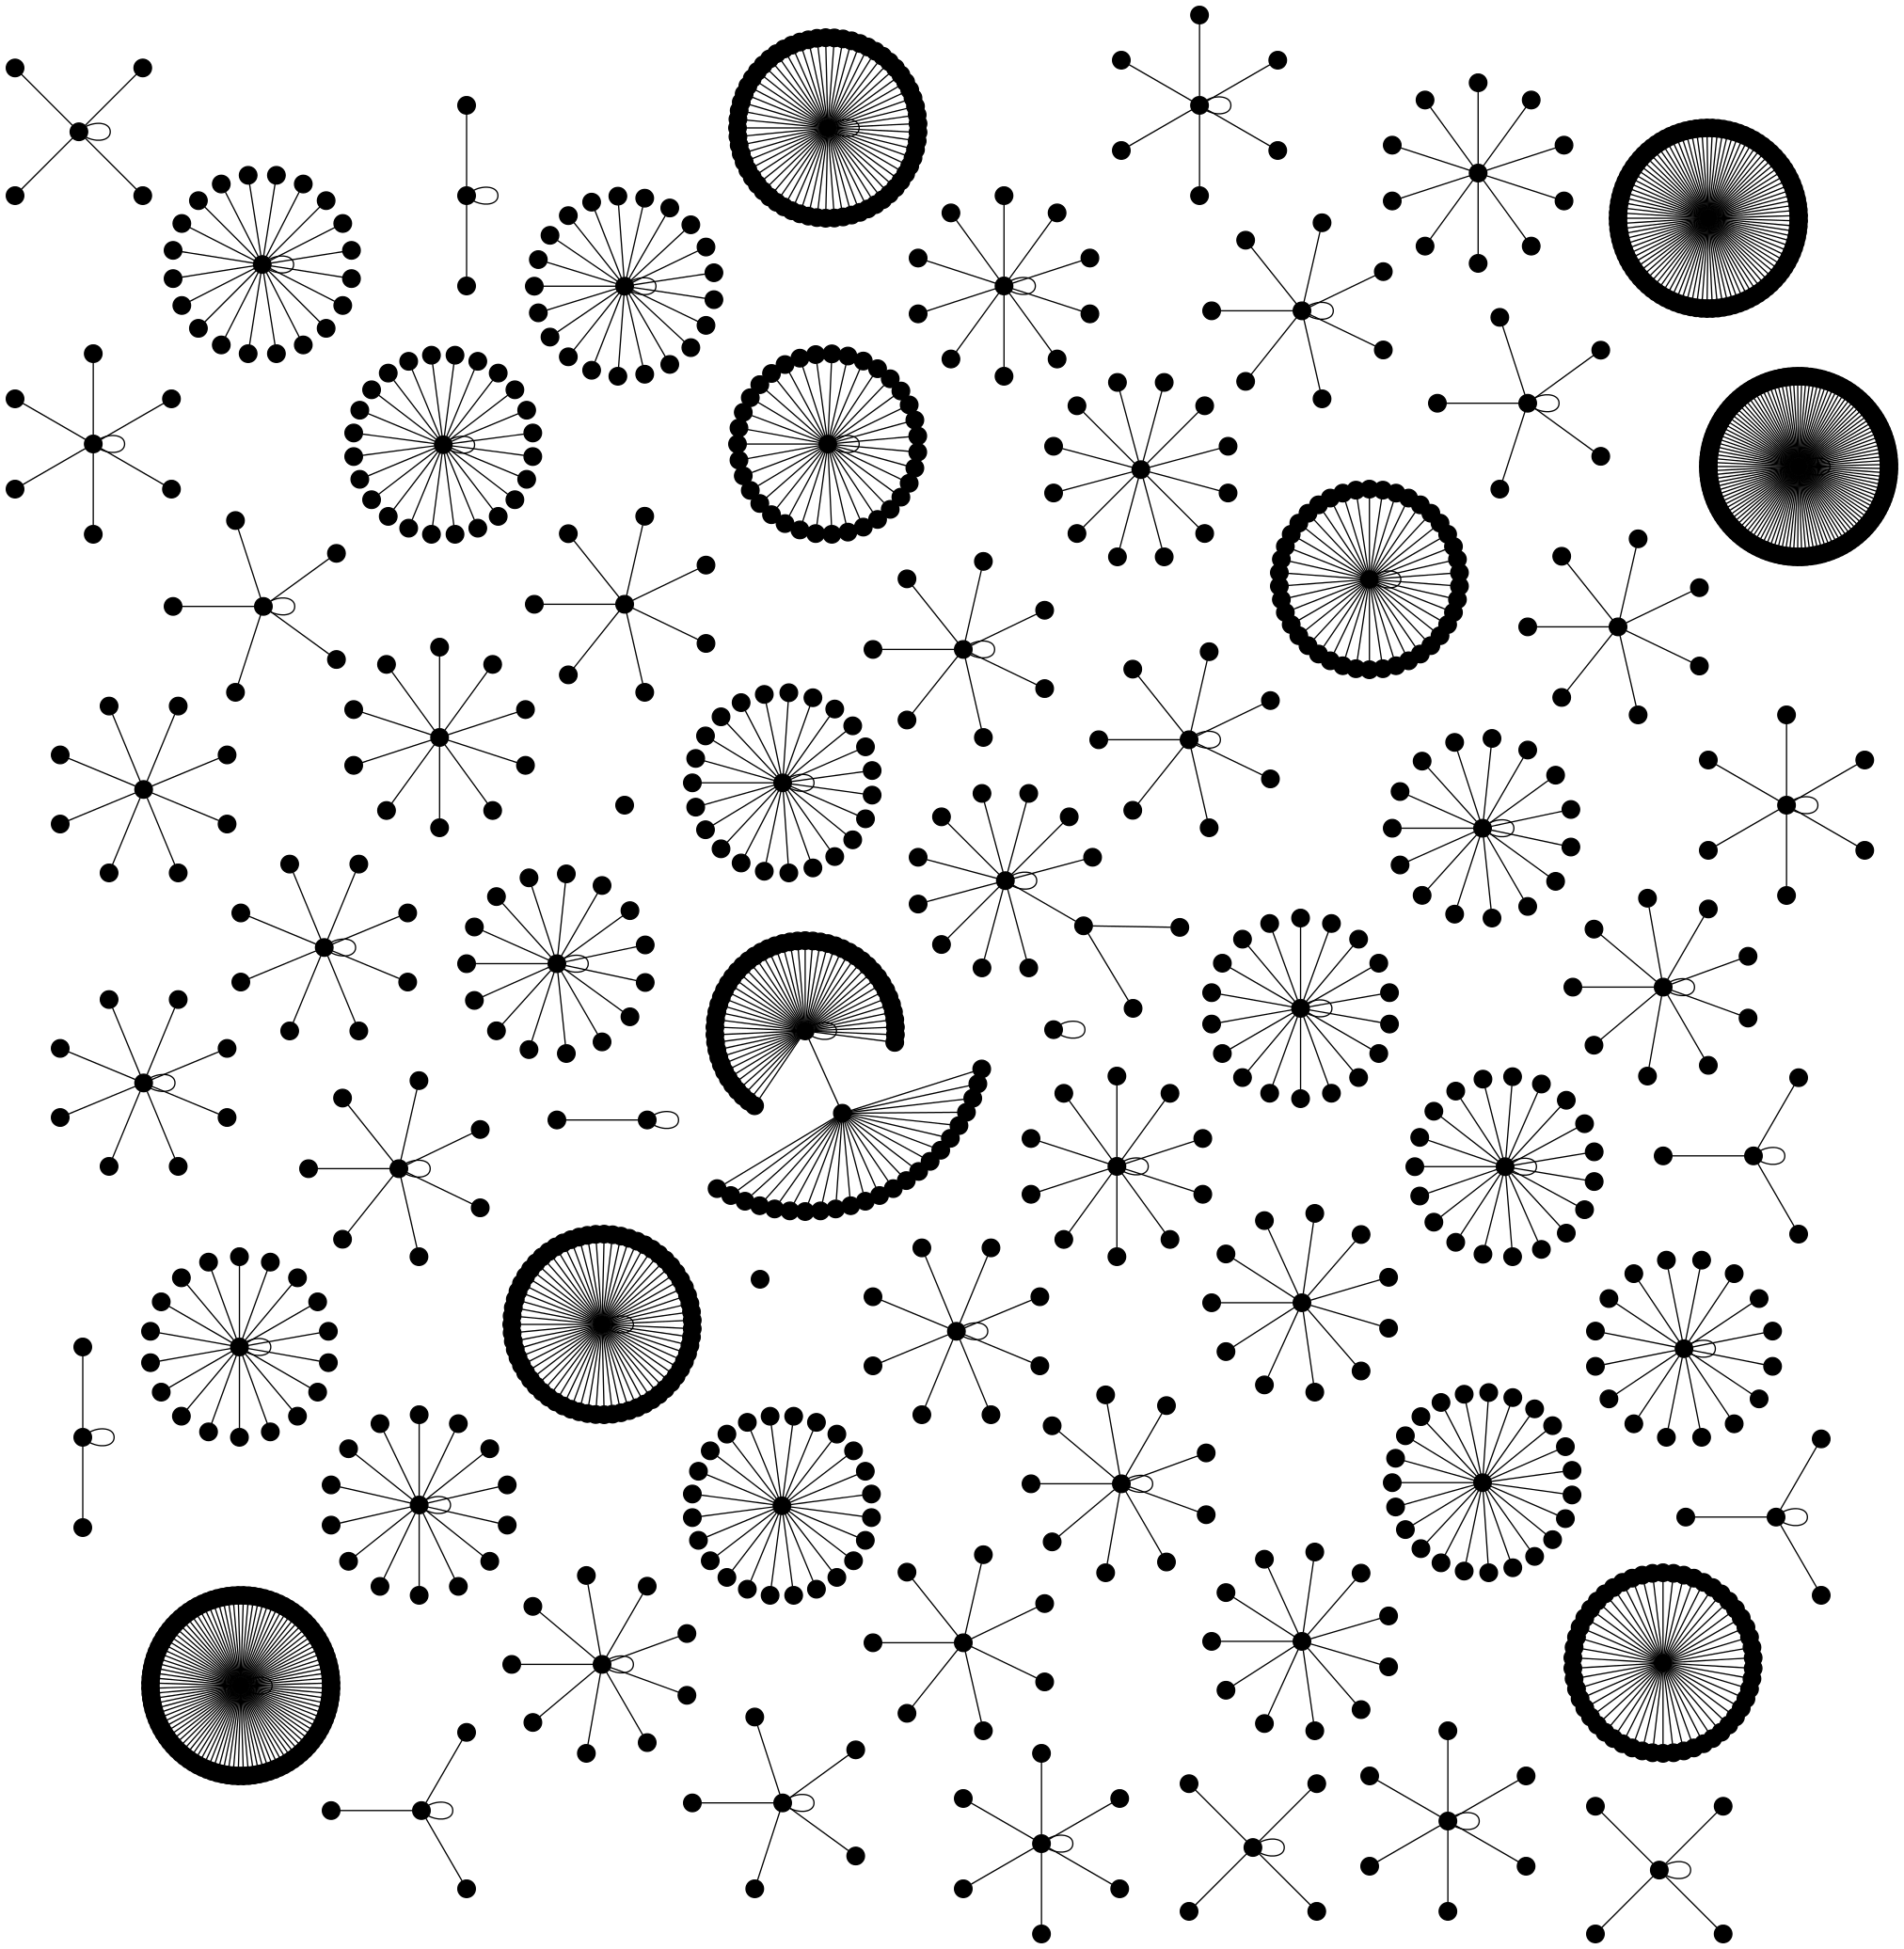
\includegraphics[scale=0.10]{img/w_directories.png}
\caption{a random generation of unrelated concepts}
\label{}
\end{figure}



\begin{figure}[htp]
\centering
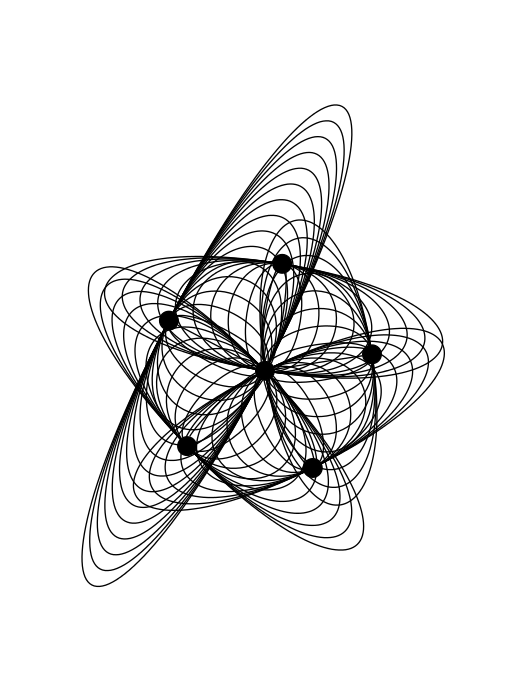
\includegraphics[scale=0.60]{img/science_fiction_directories.png}
\caption{}
\label{}
\end{figure}



\begin{figure}[htp]
\centering
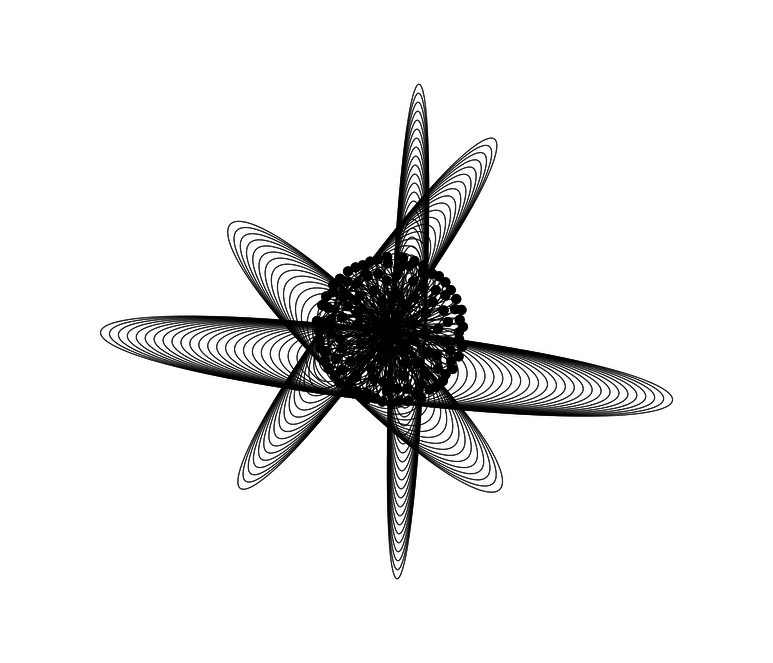
\includegraphics[scale=0.6]{1363498617__knowledge-reactor.png}
\caption{}
\label{}
\end{figure}

\end{document}

